\chapter{Introduction}
\label{chap:intro}

\section{Executive Summary}

Patients who have suffered from a stroke or a traumatic brain injury can develop
a condition called left side neglect, which is the inability of the right side
of the brain to process information that comes from the left side of the body
and can cause the patient to forget that there is a whole world to their left
side. Dr. Kate Enzler, a physical therapist at the Alexian Brothers
Rehabilitation Hospital, works with patients who have left neglect and has found
that current solutions for treating left neglect are not entirely feasible for
daily use. Our class was tasked with designing a device that could remind
patients to scan to their left in order to aid in the rehabilitation process. To
approach this challenge, we conducted research on current solutions to left
neglect and interviewed Dr. Enzler to gain further insight into the usefulness
of these solutions, which allowed us to come up with three mockups. However,
after user testing, it was found that different solutions worked best in
different contexts, so it was decided as a class that each team would design a
component of a greater “take-home kit” solution that could provide a more
thorough approach to the rehabilitation process. Our component is a feedback
device that is housed on a glasses strap and can track how far the user has
turned their head. The major components of our device include an accelerometer
gyroscope, which is able to track head movements, and an ESP-32 microcontroller,
which is able to process the data collected by the gyroscope and send it via
bluetooth to the other team’s components. The major benefit of this device is
that it allows for the personalization of the take-home kit; by tracking the
user’s head movements, the stimuli from the glasses and haptic clip can be
adjusted to turn on when the user needs to scan left and turn off once the user
has succeeded in looking all the way to their left. Therefore, this device helps
to meet the solution requirements of customizability and adjustability, and its
compactness also meets the requirement of wearability. Looking at future
development of the design, one improvement that can be made is to refine the
electronics with a custom printed circuit board so that they take up even less
surface area. In addition, the angle-determination algorithm used by the device
could be refined to make it more accurate.

\section{Introduction}

Patients who have suffered from a stroke or a traumatic brain injury can develop
a condition called left side neglect. This condition is caused by the inability
of the right side of the brain to process information that comes from the left
side of the body. Patients therefore struggle to engage with the left side of
their body (see \autoref{chap:research}). This project specifically
addresses the patients who struggle to continue turning their head past the
midline of the body. Our project partner, physical therapist Dr. Kate Enzler,
stated during the client interview that the typical patient often forgets there
is a whole world to the left side of the body. This lack of head rotation poses
everyday challenges for the patient, as they may bump into things on the left
side of them, miss information when reading, etc. (see
\autoref{chap:interviews}). The solution to this problem is preferably wearable
as per our client’s request. Since left neglect patients span a wide
demographic, the solution must be customizable not only to fit differently sized
patients, but to also work for patients with varying degrees of left neglect
(see \autoref{chap:project_def}).

The research phase of this project consisted of both primary and secondary
research. While researching the condition of left neglect, we also researched
existing solutions for the condition and their shortcomings in order to avoid
those elements in our design. Current methods of treatment include neck
vibration therapy, prism therapy, eye patching, optokinetic stimulation, and the
use of tangible stimuli to remind a patient to visually scan left. Many of these
visual stimuli are effective short-term but do not have lasting long-term
effects. Additionally, many of the products, despite being effective, required a
lot of work with the therapist in order to understand how the device worked or
what its purpose was. Many of these solutions also create a reliance on the
patients’ caregivers, limiting patient autonomy (see \autoref{chap:research}).
The goal of the product that we designed was to aid patients in
regaining their autonomy while continuing to receive cues as a reminder to
visually scan left.  Our solution is a haptic motor clip that attaches onto a
patient's hat or shirt, to a point of skin contact on the right side of their
body, which serves as a haptic stimulus to remind the patient to visually scan
left. The motor will connect via bluetooth to an app, which will control the
motor. The final part of the solution will consist of a pair of glasses that
have cue lines on the left side that guide the patients towards the left. The
glasses also have a gyroscope on them that track motion and will communicate
with the app, and turn the motor and lights off when the patient has turned
their head to a certain degree.

\begin{figure}[h]
  \centering
  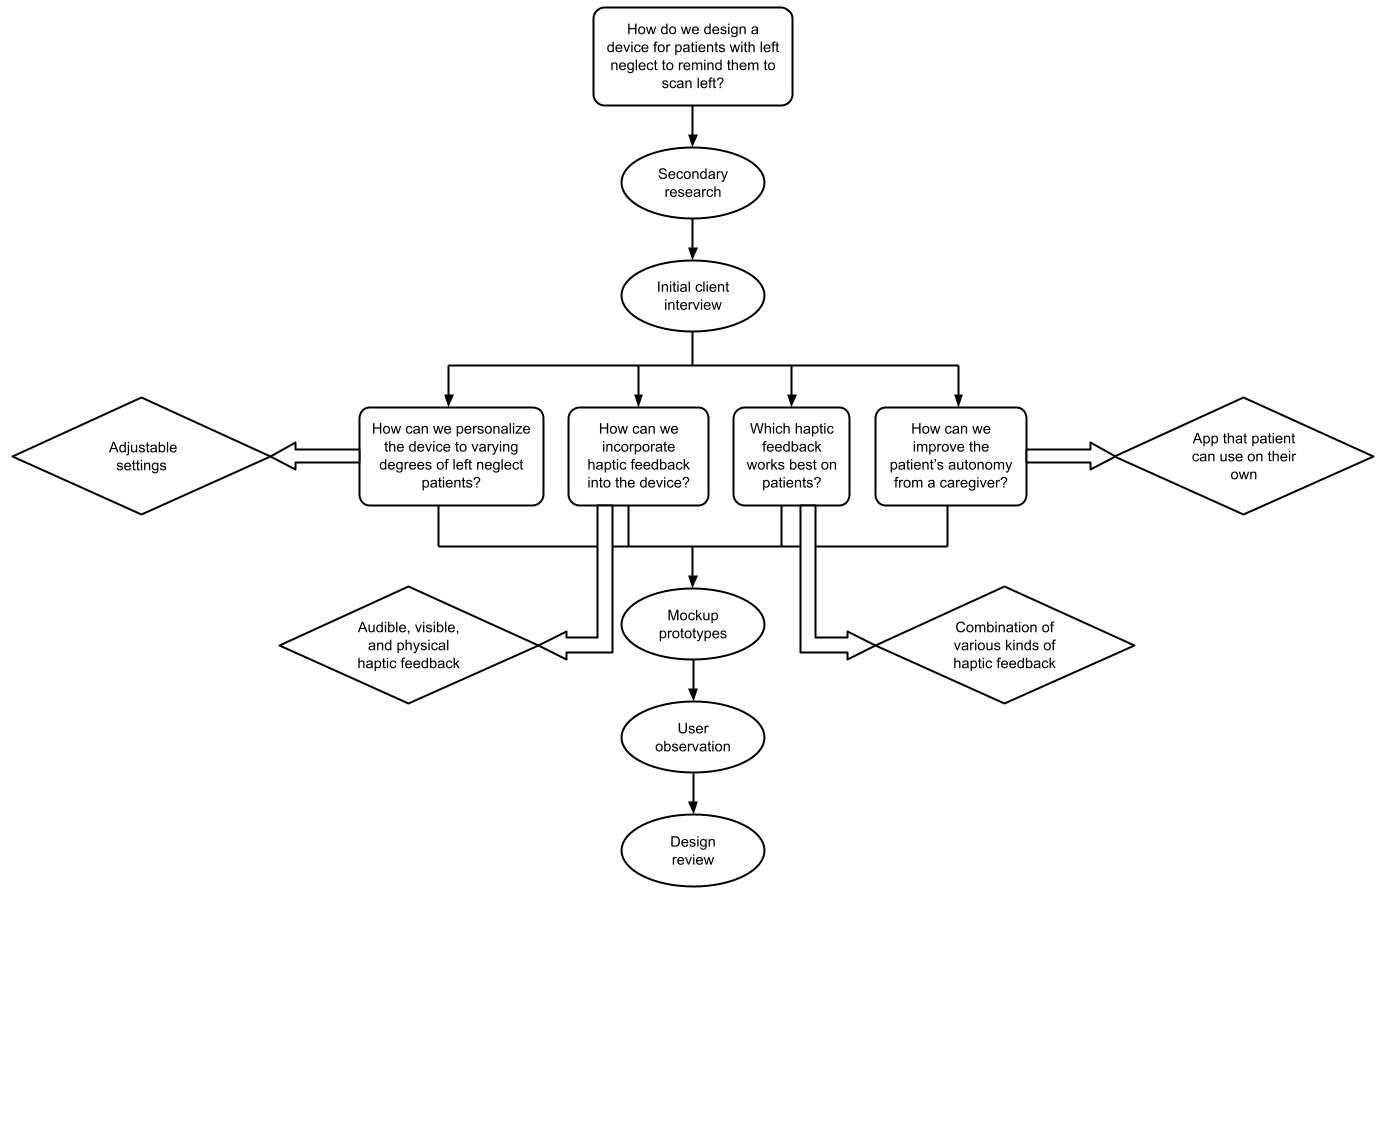
\includegraphics[width=\textwidth]{process}
  \caption[Design Process]{Flowchart that steps through a general design
    process all teams went through prior to the design review.}
  \label{fig:process}
\end{figure}

Prior to the design review, every team partook in their own separate design
process. All teams initially faced the same overarching challenge of designing a
device for patients with left neglect that will remind them to scan
left. Prompted with this question, every team delved into their own individual
secondary background research (see \autoref{chap:research}) and presented differing
questions to Dr. Kate Enzler during the client interview to gain more insight on
the problem (see \autoref{chap:interviews}). After this interview with
Dr. Enzler and the user observation (see \autoref{chap:observations}, the teams
began ideating and creating mockups that resulted in some
general similarities such as adjustable settings, a combination of audible,
visible, and physical haptic feedback, and an app that can control such
feedback. All the team’s prototypes were then brought to user testing, where
the teams learned what aspects of their prototypes did or did not function
ideally (see \autoref{chap:feedback}). It was at the design review that the entire
section realized all teams had versions of the same general prototype idea
(see \autoref{fig:process}).
Through this realization, we collectively decided upon assigning each
team to oversee and create one design to eventually combine all four separate
designs into one system rather than presenting four versions of the same design
to the client. 

\section{Design Requirement Status}

Each of the products individually serve a greater purpose to fulfill the design
requirements our product partner provided. The greater design requirements are
as follows; Produce a product that is durable, simple, and affordable, that
reminds a patient with left neglect to scan to the left. With our original
individual groups we were struggling to provide for the full design requirements
but as a collective with four different roles we were able to effectively meet
each major requirement. The individual components of the product include a pair
of glasses, a feedback device, a clip, and an app. Each team has been assigned
one component to work on for the remainder of the project but all the components
work together in order to create one product that meets all the
requirements. The Glasses team was able to meet the requirement of having a
reminder to help the patients look left. The lights on the glasses serve as a
constant visual reminder for those wearing the device. This paired with the
haptics provide a range of stimuli to remind the user as the haptics headband
works to also fulfill the same design requirement. These two components together
fulfill the most important part of the design requirements and provide a solid
base for the rest of the components to build upon. 

Next comes the gyroscope which will be taking the data from the two reminding
components and relaying it to the final component, the app. This helps to keep
the project simple and adaptable so the user can track their progress and
determine if the product is helping with their left neglect. This feedback is
crucial to determining the efficacy of the project. The app works in tandem with
the gyroscope to take in the data from the patient and provide a simple and
usable interface to interact with. 

All of these components help together to assist the patient with scanning left
and provides them with feedback on the progress from their time using the
product (see \autoref{fig:system}). 

\begin{figure}[h]
  \centering
  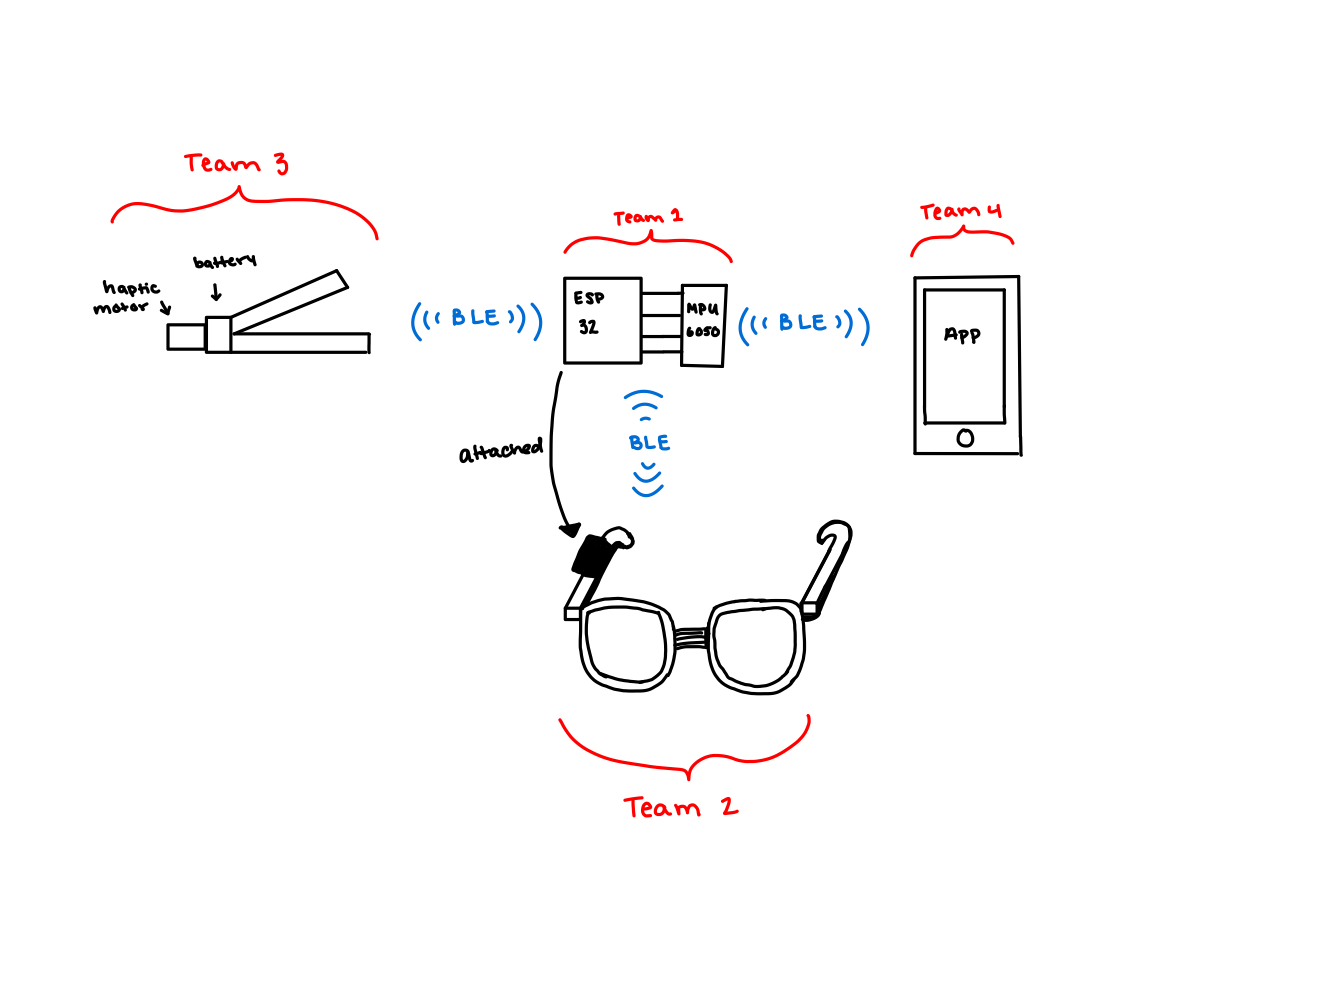
\includegraphics[width=\textwidth]{system}
  \caption[System Diagram]{Integration diagram that shows how each component
    works together and which teams are involved in what parts.}
  \label{fig:system}
\end{figure}

%%% Local Variables:
%%% mode: latex
%%% TeX-master: "../final_report"
%%% End:
